\section{Strategia di swing-up}
Per lo swing-up, uso il metodo di Lyapunov così come descritto in [Astrom Furuta swinging up a pendulum by energy control].
%todo ref
Quello che voglio fare è:

\begin{enumerate}
    \item Studiare l'effetto del controllo sull'energia del solo pendolo
    %
    \item Trovare una CLF per il pendolo che permetta lo swing-up.
\end{enumerate}
%todo glossary clf

\subsection{Energia del pendolo}
\label{subsec:energia-pendolo}
L'energia del solo pendolo è data da:
\begin{equation}
    E = T + V = \frac 1 2 I \dot \theta^2 + mgL(\cos\theta-1)
    \label{eq:energia-pendolo}
\end{equation}
dove ho scelto il potenziale in modo che si annulli quando $\theta=0$. Voglio studiare che effetto ha un accelerazione del perno sul pendolo. Posso farlo risolvendo l'equazione di eulero:
\begin{equation*}
    \frac {\partial^2} {\partial t \partial \dot \theta} \mathcal L - \frac \partial {\partial \theta} \mathcal L = -L ma \cos \theta
\end{equation*}
dove compare la Lagrangiana $\mathcal L$ del solo pendolo e a secondo membro compare il momento torcente che l'accelerazione $a$ imprime al pendolo. Il risultato è che l'effetto dell'accelerazione $a$ del carrello sul pendolo è dato dall'equazione:
\begin{equation}
    I \ddot \theta - mgL\sin \theta + maL \cos \theta = 0
    \label{eq:moto-pendolo}
\end{equation}
\todo{qui ci starebbe bene un disegnino...}
%todo qui bisogna sistemare un po' i simboli
e posso usare le due equazioni \eqref{eq:moto-pendolo} e \eqref{eq:energia-pendolo} per calcolare la variazione di energia istantanea che produce l'accelerazione $a$ lungo la traiettoria del moto. Calcolo:
\begin{equation}
    \begin{aligned}
        \partiald t E
        &= \partiald t \left(\frac 1 2 I \dot \theta ^2 + mgL \cos \theta  \right) \\
        &= I \dot \theta \ddot \theta - mgL \sin \theta \cdot \dot \theta \\
        &= -maL \cos \theta \cdot \dot \theta
        .
        \label{eq:effetto-energia}
    \end{aligned}
\end{equation}
Osservando la \eqref{eq:effetto-energia} posso ricavare una strategia di controllo rudimentale, schematizzata in figura \ref{fig:energy-control}:
\begin{itemize}
    \item Se l'energia è minore di $0$, aggiungo energia al massimo rate possibile per il sistema: $a = a_{\max}\sign{\dot \theta \cos \theta}$.
    \item Se l'energia è maggiore di $0$, tolgo energia al massimo rate possibile per il sistema: $a = -a_{\max}\sign{\dot \theta \cos \theta}$.
\end{itemize}
Una strategia di questo tipo è detta \emph{bang-bang} e ha il vantaggio di essere
la strategia che impiega mento tempo a raggiungere l'obiettivo,
come conseguenza del principio di Pontryagins [qui devo vedere se spiegare primna il principio. Questa cosa comunque la spiega sempre Astrom in swing up with energy control...].
Tuttavia, questa strategia è estremamente sensibile al rumore,
in quanto piccole variazioni dell'energia creano discontinuità nel controllo.

\begin{figure}
    \centering
    \begin{subfigure}[b]{0.48\textwidth}
        \centering
        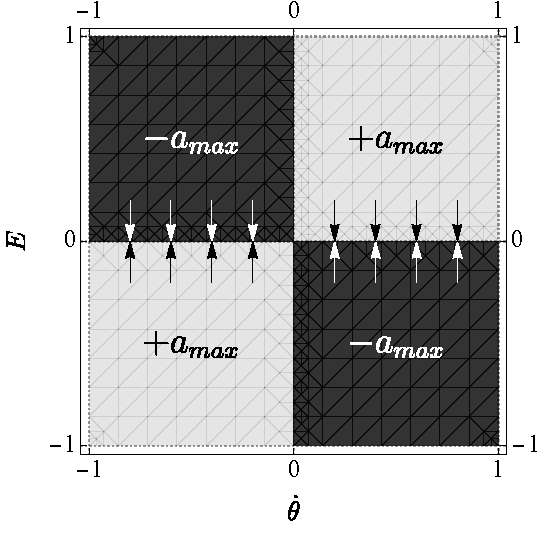
\includegraphics[width=\textwidth]{assets/energy-control1}
        \caption{aaaaa}
    \end{subfigure}
    \hfill
    \begin{subfigure}[b]{0.48\textwidth}
        \centering
        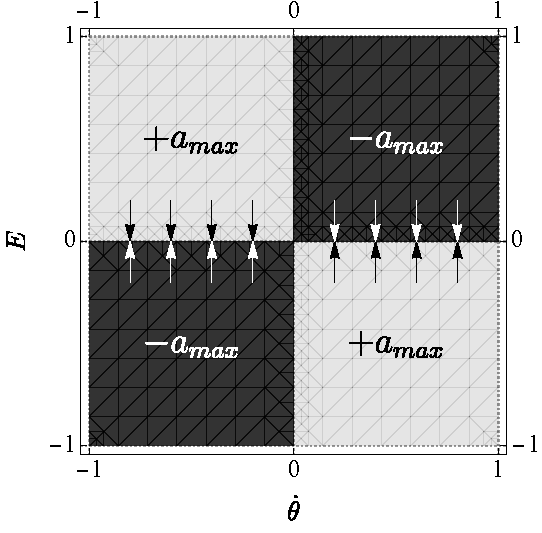
\includegraphics[width=\textwidth]{assets/energy-control2}
        \caption{bbbbb}
    \end{subfigure}
    \caption{Schema del sistema.} %todo
    \label{fig:energy-control}
\end{figure}

\subsection{Funzione di Lyapunov e CLF}
\paragraph{Si può fare di meglio,} impiegando una CLF per ricavare una strategia di controllo. Questo permette sia di avere una strategia di controllo smooth, sia di dimostrare rigorosamente che il sistema raggiungerà l'equilibrio cercato, grazie ai teoremi ??\todo{qui dovrò citare teoremi scritti prima su controllabilità con lyapunov}.
Devo trovare una strategia di controllo $a$ e una funzione di Lyapunov $V$ che rispettino le condizioni di [riferimento alla definizione di funzione di lyapunov \todo{teoria}].
Per cercare $a$ mi ispiro alle considerazioni fatte a fine paragrafo \ref{subsec:energia-pendolo}. La funzione che si presta di più è la tangente tangente iperbolica, per via dell'effetto soglia:
\begin{equation}
    a = a_{\max} \tanh(E \dot \theta \cos \theta).
    \label{eq:control-strategy-test}
\end{equation}
Questa strategia è schematizzata in figura \ref{fig:energy-control-smooth}.
\begin{figure}
    \centering
    \begin{subfigure}[b]{0.48\textwidth}
        \centering
        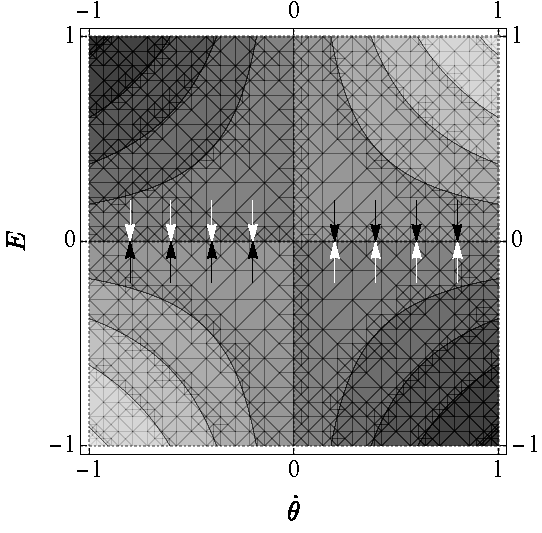
\includegraphics[width=\textwidth]{assets/energy-control3}
        \caption{aaaaa}
    \end{subfigure}
    \hfill
    \begin{subfigure}[b]{0.48\textwidth}
        \centering
        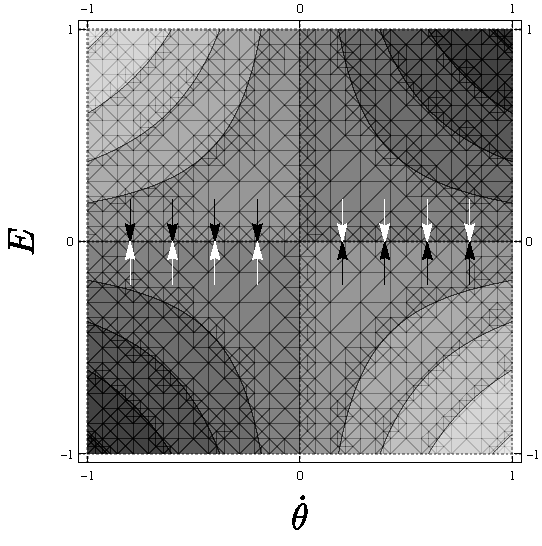
\includegraphics[width=\textwidth]{assets/energy-control4}
        \caption{bbbbb}
    \end{subfigure}
    \caption{Schema del sistema.} %todo
    \label{fig:energy-control-smooth}
\end{figure}

Ora, se definisco $V$ come:
\begin{equation}
    V = \frac 1 2 E^2.
    \label{eq:lyapunov-energy}
\end{equation}
È facile dimostrare che ho trovato una CLF. Infatti, se calcolo la detivata di $V$ e sostituisco l'espressione di $a$ appena definita:
\begin{equation}
    \begin{aligned}
        \partiald t V &= \partiald t \left( \frac 1 2 \dot E^2\right) \\
        &=  E \dot E \\
        &=  E (-maL \dot \theta \cos \theta) \\
        &= -mLE\dot \theta \cos \theta \cdot a_{\max} \tanh(E \dot \theta \cos \theta).
    \end{aligned}
    \label{eq:lyapunov-energy}
\end{equation}
Per dimostrare che questa è una CLF devo mostrare che $V'(t) < 0 q.o.$ e ciò è banale visto che la tangente iperbolica preserva il segno. Di conseguenza la funzione è negativa a patto che:
\begin{itemize}
    \item $\dot \theta \neq 0$
    \item $\cos \theta \neq 0$
\end{itemize}
tuttavia, nessuna di queste configurazioni è stabile per il sistema\footnote{$\dot \theta = 0$ è stabile se $\theta = \{0, \pi\}$, ma $\theta = 0$ è il punto a cui vogliamo arrivare e $\theta = \pi$ è il punto di partenza; basta quindi fornire un impulso iniziale al sistema e questo inizierà a muoversi.}, quindi possiamo affermare che $V$ tenderà a zero e l'angolo tenderà a $\theta = 0$.
È opportuno sottolineare che questa strategia non tiene in considerazione la posizione del carrello lungo la rotaia.
È quindi necessario passare alla strategia \ref{sec:strategia-stabilizzazione}
una volta che il pendolo raggiunge la verticale.